\documentclass[letterpaper, 11pt]{article}
\usepackage{amsmath}
\usepackage{amssymb}
\usepackage{float}
\usepackage{inputenc}
\usepackage[left=2cm, right=2cm, top=2cm, bottom=2cm]{geometry}
\usepackage{graphicx}
\usepackage{float}
\usepackage{caption}
\usepackage{extarrows}
\usepackage{xcolor}
\usepackage{lscape}
\usepackage{pdflscape}
\usepackage{pdfpages}
\usepackage{multicol}
\usepackage{leftindex}
\usepackage{algorithm2e}
\SetKwComment{Comment}{/* }{ */}
%\RestyleAlgo{ruled}
\usepackage{mathtools}
\usepackage{hyperref}
\hypersetup{
    colorlinks=false,
    }

% Listings
\usepackage{listings}
\usepackage{color}
\definecolor{mygreen}{rgb}{0,0.6,0}
\definecolor{mygray}{rgb}{0.5,0.5,0.5}
\definecolor{mymauve}{rgb}{0.58,0,0.82}

\lstset{
  backgroundcolor=\color{white},   % choose the background color; you must add \usepackage{color} or \usepackage{xcolor}; should come as last argument
  basicstyle=\small\ttfamily,        % the size of the fonts that are used for the code
  breakatwhitespace=false,         % sets if automatic breaks should only happen at whitespace
  breaklines=true,                 % sets automatic line breaking
  captionpos=t,                    % sets the caption-position to bottom
  commentstyle=\color{mygreen},    % comment style
  deletekeywords={...},            % if you want to delete keywords from the given language
  escapeinside={\%*}{*)},          % if you want to add LaTeX within your code
  extendedchars=true,              % lets you use non-ASCII characters; for 8-bits encodings only, does not work with UTF-8
  firstnumber=1,                % start line enumeration with line 1000
  frame=false,	                   % adds a frame around the code
  keepspaces=true,                 % keeps spaces in text, useful for keeping indentation of code (possibly needs columns=flexible)
  keywordstyle=\color{blue},       % keyword style
  language=Python,                 % the language of the code
  morekeywords={*,...},            % if you want to add more keywords to the set
  numbers=none,                    % where to put the line-numbers; possible values are (none, left, right)
  numbersep=5pt,                   % how far the line-numbers are from the code
  numberstyle=\tiny\color{mygray}, % the style that is used for the line-numbers
  rulecolor=\color{black},         % if not set, the frame-color may be changed on line-breaks within not-black text (e.g. comments (green here))
  showspaces=false,                % show spaces everywhere adding particular underscores; it overrides 'showstringspaces'
  showstringspaces=false,          % underline spaces within strings only
  showtabs=false,                  % show tabs within strings adding particular underscores
  stepnumber=5,                    % the step between two line-numbers. If it's 1, each line will be numbered
  stringstyle=\color{mymauve},     % string literal style
  tabsize=4,	                   % sets default tabsize to 2 spaces
  title=\lstname                   % show the filename of files included with \lstinputlisting; also try caption instead of title
}


% NewCommands
\newcommand{\peq}{ \mathrel{+}= }
\newcommand{\muleq}{ \mathrel{*}= }
\newcommand{\sign}{\,\text{sign}}
\newcommand{\bm}[1]{\begin{bmatrix} #1 \end{bmatrix}}
\newcommand{\lx}[2]{\leftindex #1 {#2}}
\newcommand{\norm}[1]{\left\lvert #1 \right\rvert}
\newcommand{\abs}[1]{\norm{#1}}
\newcommand{\itbf}[1]{\textit{\textbf{#1}}}
\newcommand{\mdet}[1]{\norm{\begin{matrix} #1 \end{matrix}}}
\newcommand{\lr}[1]{\left( #1 \right)}
\newcommand{\sat}{\,\text{sat}}



\title{Identification and Control of Multirotor Actuator Dynamics with RPM feedback}
\author{Sesha Charla}
\date{\today}


\begin{document}
\maketitle
\tableofcontents
\newpage
\
% ==============================================================================
\newpage
\section{Control Model and Input}
From the results of system modelling and identification, we have the non-linear
model of the system and the corresponding model parameter estimates.

\begin{equation}\label{eqn::nl_model}
    J \dot \omega + b_m \omega + C_D \omega^2 + M_f \delta v = V_{in} b_m u_\omega + V_{in}^2 (1 + \delta v) C_D u_\omega^2
\end{equation}


\begin{table}[H]
    \centering
    \begin{tabular}{c l l c}
        \hline \hline
        Parameter & Value & & $\sigma$            \\ \hline \hline
        $C_T$ & $7.2581 \times 10^{-06}$ & $N/(rad/s)^2$   & $4.4522 \times 10^{-8}$ \\
        $C_D$ & $3.6088 \times 10^{-08}$ & $N.m/(rad/s)^2$ & $1.3964 \times 10^{-9}$ \\
        $b_m$ & $0.0$                    & $N.m/(rad/s)$   & $4.6003 \times 10^{-6}$  \\
        $M_f$ & $1.3135 \times 10^{-3}$  & $N.m$           & $4.5277 \times 10^{-3}$ \\
        $J$   & $3.2238 \times 10^{-6}$   & $Kg.m^2$        & $7.0053 \times 10^{-6}$ \\
        \hline \hline
    \end{tabular}
    \caption{Summary of parameter estimates from static and small-perturbation experiments}
    \label{tab::parm_ests}
\end{table}

From parameter estimates (Table~\ref{tab::parm_ests}), it can be seen that the
estimate of total 'damping' factor $( b_m )$ is zero. Thus, the linear term of
the control input in the RHS of eqn.~\ref{eqn::nl_model} can be ignored.
Let $u = u_\omega ^2 $ be the control input to the system for which we are going
to design the feedback controller. Incorporating the above two assumptions into
eqn.~\ref{eqn::nl_model}, we have the control form of the model:
\begin{equation} \label{eqn::control_form}
    J \dot \omega + b_m \omega + C_D \omega^2 + M_f \delta v = V_{in}^2 (1 + \delta v) C_D u
\end{equation}

%===============================================================================

%===============================================================================
\newpage
\section{Characterizing the Effects of Modelling Uncertainities and Assumptions}
The modelling uncertainities due to the uncertainities in the input definition
and the parameter estimates affect the tracking performance of the controller.
The primary sources of the uncertainities are as follows:
\begin{enumerate}
    \item Uncertainities due to the input definition.
    \begin{enumerate}
        \item Uncertainities caused by neglecting the linear term in the input based on
        the assumptions $b_m = 0 \implies V_{in} b_m u_\omega = 0$.
        \item Effects of non-zero and slowly varying $\delta v$.
    \end{enumerate}

    \item Uncertainities in the model parameter estimates.
\end{enumerate}

The effects of the uncertainities are determined by the relative error in the
prediction from the nominal model and the model with only that particular uncertainity.

\subsection{Effects of non-zero $b_m$}
From the simulink model the uncertainity in $b_m$ does'nt effect the prediction
error significantly. A $3 \sigma$ variation in $b_m$ produced less than $1\%$
relative error in the prediction. Thus, $b_m$ can be completely neglected out of
the non-linear model without significant prediction errors.

\begin{figure}[H]
\begin{minipage}{0.49\textwidth}
    \begin{figure}[H]
        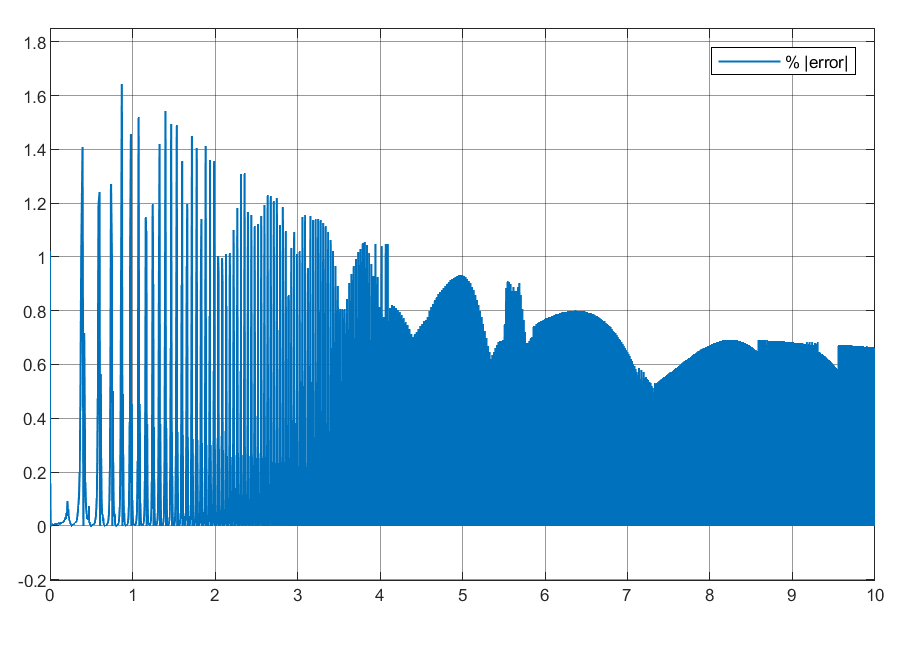
\includegraphics[width = \textwidth]{figs/par_var/3_sig_bm.eps}
        \caption{$\%$ error for $3 \sigma$ variation in $b_m$}
    \end{figure}
\end{minipage}
\begin{minipage}{0.49\textwidth}
    \begin{figure}[H]
        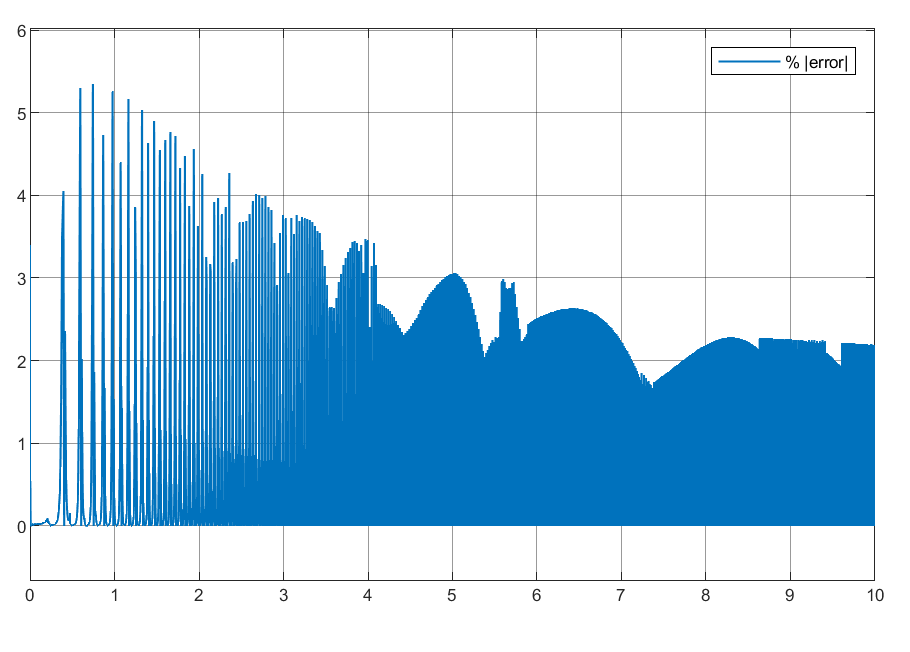
\includegraphics[width = \textwidth]{figs/par_var/10_sig_bm.eps}
        \caption{$\%$ error for $10 \sigma$ variation in $b_m$}
    \end{figure}
\end{minipage}
\end{figure}

\subsection{Effects of non-zero $\delta v$}
$\delta v$ significantly effects the prediction error as it is effectivly
changes the input-gain and also introduces un-compensated friction into the
system.
\begin{figure}[H]
\begin{minipage}{0.49\textwidth}
    \begin{figure}[H]
        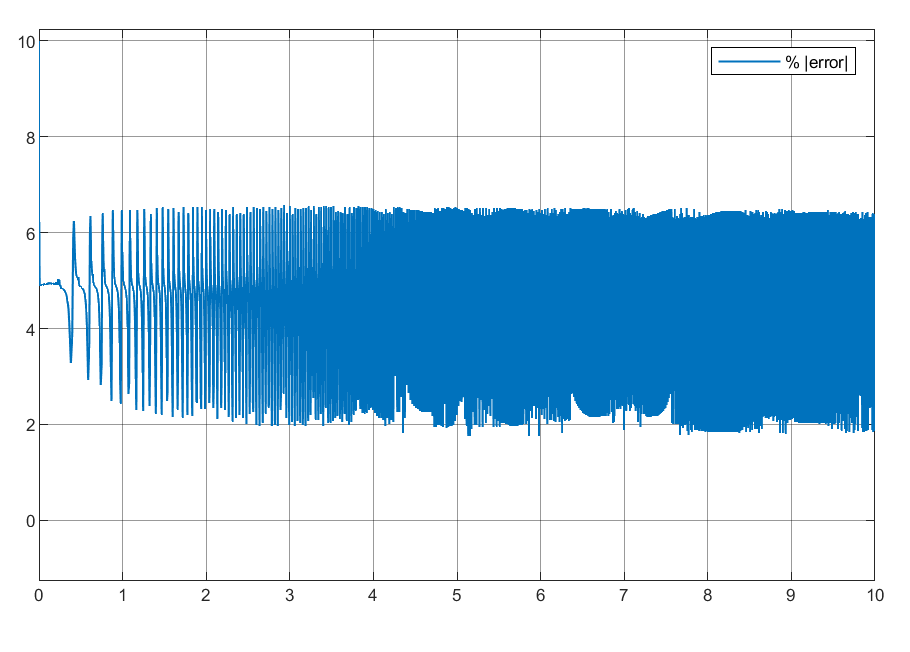
\includegraphics[width = \textwidth]{figs/par_var/1_del_v.eps}
        \caption{$\%$ error $\delta v = 0.1$}
    \end{figure}
\end{minipage}
\begin{minipage}{0.49\textwidth}
    \begin{figure}[H]
        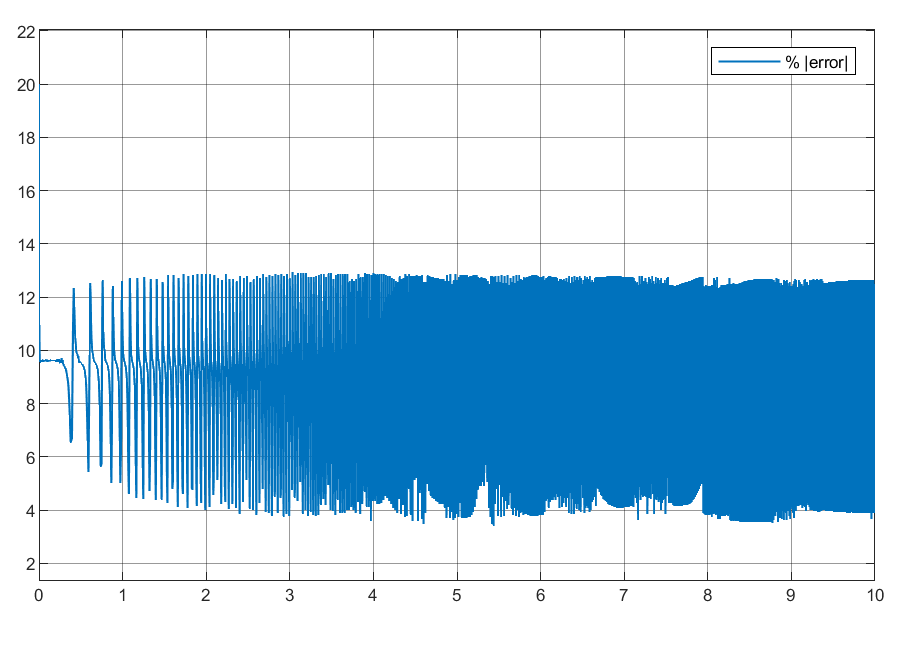
\includegraphics[width = \textwidth]{figs/par_var/2_del_v.eps}
        \caption{$\%$ error for $\delta v = 0.2$}
    \end{figure}
\end{minipage}
\end{figure}


\subsection{Effects of model-parameter estimation errors}
The parameter $J, C_D$ effect the prediction errors to the same order of
magnitude to their estimation errors. The figures bellow show the effect of
$10\%$ estimation errors in their parameters.

\begin{figure}[H]
\begin{minipage}{0.49\textwidth}
    \begin{figure}[H]
        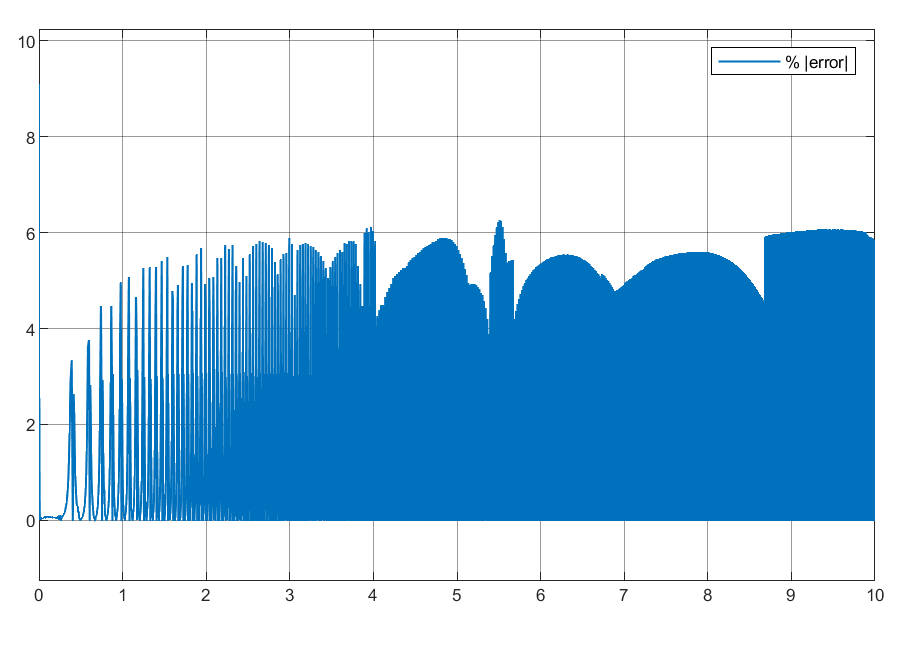
\includegraphics[width = \textwidth]{figs/par_var/j.eps}
        \caption{$\%$ error for $10\%$ error in J}
    \end{figure}
\end{minipage}
\begin{minipage}{0.49\textwidth}
    \begin{figure}[H]
        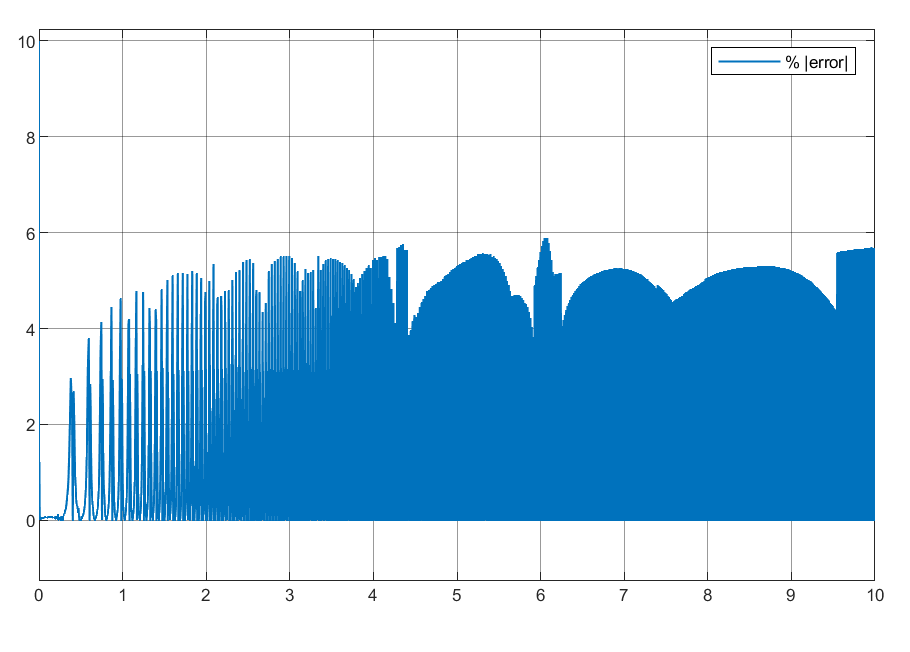
\includegraphics[width = \textwidth]{figs/par_var/c_d.eps}
        \caption{$\%$ error for $10\%$ error in $C_D$}
    \end{figure}
\end{minipage}
\end{figure}

The effect of $M_f$ is indirectly effects $\delta v$. These errors have to be
lumped together for estimation.
    \begin{figure}[H]
        \centering
        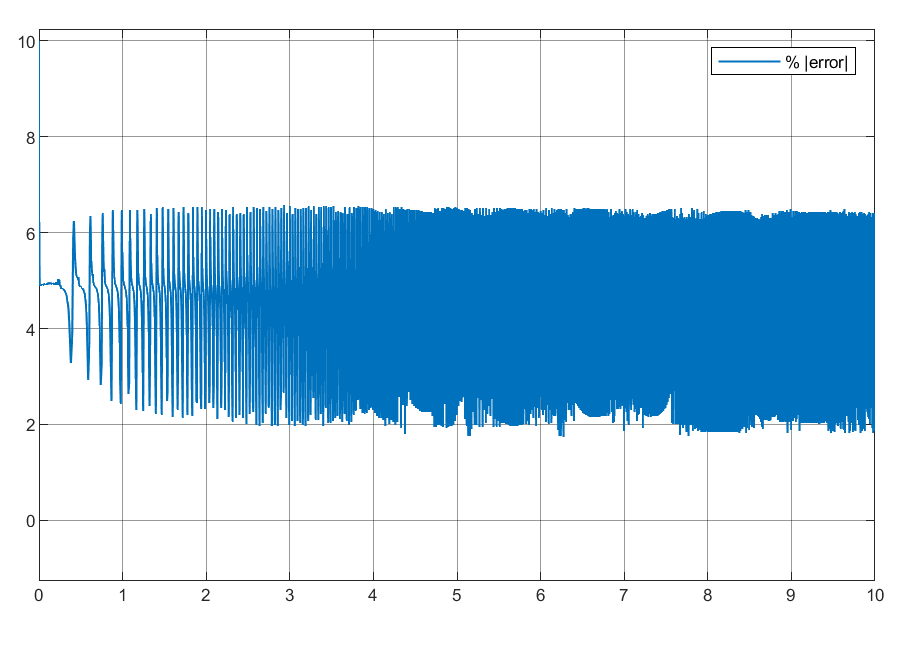
\includegraphics[width = 0.49\textwidth]{figs/par_var/m_f.eps}
        \caption{$\%$ error for $10\%$ error in $M_f$ with $\delta v=0.1$}
    \end{figure}


\subsection{Conclusion}
Thus from above analysis, we conclude following:

\begin{enumerate}
\item The model parameters that significantly effect the tracking performance
are (in the order of their infulunce): $1) \delta v, \, 2) M_f, \, 3)J, \, 4) C_D$
\item The linear damping factor of the motor $b_m$ doesn't significantly effect
the tracking performance of the system with-in it's estimation error. Hence, it can be removed from model simplifiying the model structure and the number of
model parameters to be estimated. Further, this analysis justifies the
assummption used to arrive at the control form \ref{eqn::control_form}. Thus, eqn. (\ref{eqn::control_form}) becomes:
\end{enumerate}

\begin{equation}\label{eqn::no_bm_ctrl_form}
    J \dot \omega + C_D \omega^2 + M_f \delta v = V_{in}^2 (1 + \delta v) C_D u_\omega^2
\end{equation}

%===============================================================================
\newpage
\section{Reference Trajectory Generation Problem}

%===============================================================================
\newpage
\section{Direct Adaptive Robust Control Design (DARC)}
In this section, a discontinuous projection based direct adaptive robust control
is implemented. Though the parameter convergence and tracking performance is
slightly lower than the  more advanced designs such as IARC and DIARC, DARC has
the advantage of being least computationally complex among them, resulting in
faster sampling times in resource limited scenarios.

\subsection{Control Input Design}
Let, the total control input be the sum of the following inputs:
\begin{align*}
    u &= u_a + u_s \qquad u_s = u_{s_1} + u_{s_2}
\end{align*}
%===============================================================================
\subsubsection{Model compensation input design with parameter adaption ($u_a$)}
Let, From eqn.~\ref{eqn::error_dyn}, we chose $u_a$ such that it compensates for
the error dynamics, i.e.,
\begin{align*}
    u_a &= - \pmb \phi^T  \hat{\pmb{\theta}} \\
    \text{where, } \qquad &\\
    \dot{\hat{\pmb{\theta}}} &= Proj_{\hat{\pmb{\theta}}}\lr{\Gamma \pmb \phi s}\\
\end{align*}
Where $\Gamma$ is a positive definite, diagonal adaption rate matrix.

We define, \itbf{Discontinuous projection mapping} $Proj()$ for a vector as follows:
\begin{align*}
    Proj_{\hat{\pmb\theta}} (\bullet) &= \bm{Proj_{\hat \theta_1}(\bullet_1), &
                                        Proj_{\hat \theta_2}(\bullet_2), &
                                        \hdots, &
                                        Proj_{\hat \theta_n}(\bullet_n)}\\
    Proj_{\hat \theta_i}(\bullet_i) &= \begin{cases}
        0 & \text{if } \begin{cases}
                        \hat \theta_i &= \hat \theta_{i_{min}} \text{  and  } \bullet_i < 0\\
                        \hat \theta_i &= \hat \theta_{i_{max}} \text{  and  } \bullet_i > 0\\
                       \end{cases}\\
        \bullet_i & \text{otherwise}
    \end{cases}
\end{align*}
The above mapping has the following properties:
\begin{itemize}
    \item[$P_1$:] $\quad \hat{\pmb \theta} \in \bar \Omega_{\theta}=\{\hat{\pmb \theta} : \theta_{i_{min}} \leq \hat \theta_i \leq \theta_{i_{max}} \; \forall i\} \; \forall t$

    \item[$P_2$:] $\quad \tilde{\pmb{\theta}} \left[ \Gamma^{-1}
    Proj_{\hat{\pmb\theta}} \lr{\Gamma \pmb \phi s} - \phi s \right] \leq 0 \:
    \forall t \qquad [\tilde{\pmb{\theta}} = \hat{\pmb\theta} - \pmb \theta]$
\end{itemize}

%===============================================================================

\subsubsection{Robust feedback control input design}
Substituting $u_a$ in eqn.~\ref{eqn::error_dyn}:
\begin{align*}
    \theta_1 \dot s &= -\pmb \phi^T \hat{\pmb \theta} + \pmb \phi^T \pmb \theta + \Delta + u_{s_1} + u_{s_2}\\
    \text{Let,  } u_{s_1} &= -k_p s & & [\text{Proportional Feedback}]\\
    \text{and  } \tilde{\pmb\theta} &= \hat{\pmb \theta} - \pmb \theta\\
    \implies \theta_1 \dot s + k_p s &= u_{s_2} - \pmb \phi^T \tilde{\pmb \theta} + \Delta\\
\end{align*}
Let $- \pmb \phi^T \tilde{\pmb \theta} + \Delta$ be bounded by $h(\omega, t)$,
i.e.,
\begin{align*}
    h(\omega, t) &\geq   - \pmb \phi^T \tilde{\pmb \theta} + \Delta  \quad \forall t\\
    \implies h &= \abs{\pmb \phi^T} \tilde{\pmb \theta}_M + \abs{\Delta}\\
               &= \abs{\pmb \phi^T} \tilde{\pmb \theta}_M + \Delta_M \qquad
                \tilde{\pmb \theta}_M = \pmb \theta_{max} - \pmb \theta_{min}\\
\end{align*}

Use sliding mode control law for $u_{s_2}$:
\begin{align*}
    u_{s_2} &= S(h \sign(s))\\
    \text{Where,  } \qquad &\\
    S(h \sign(s)) &= h \sat \lr{ \frac{h}{4 \varepsilon} s} &[\text{Smoothing function}]\\
    \sat (x) &= \begin{cases}
        x  & \text{if  } \abs{x} \leq   1\\
        \sign(x) &  \text{otherwise}
    \end{cases}
\end{align*}
The above defined smoothing function, $S(.)$, has the following properties:

\begin{itemize}
\item[$P_3$:] $s S(h \sign(s)) = s h \sat \lr{\frac{h}{4 \varepsilon} s} \geq
0 \qquad $ $\because$ $s$ and $\sat \lr{\frac{h}{4 \varepsilon} s}$ have the
same sign.

\item[$P_4$:] $s \left[h \sign(s) - S(h\sign(s)) \right]$ is bounded.\\
\itbf{proof:}
\begin{align*}
    s \left[h \sign(s) - S(h\sign(s)) \right] &= s \left[h \sign(s) - h \sat \lr{\frac{h}{4 \varepsilon} s} \right]
\end{align*}
\begin{enumerate}
\item Outside the boundary layer, i.e., $\lr{\abs{s} > \frac{4 \varepsilon}{h}
}$:
\begin{align*}
    sh \sign(s) - s h \sat \lr{\frac{h}{4 \varepsilon} s} &= h \abs{s} - h\abs{s} = 0
\end{align*}

\item Inside the boundary layer, i.e., $\lr{\abs{s} < \frac{4 \varepsilon}{h}}$
\begin{align*}
    sh \sign(s) - s h \sat \lr{\frac{h}{4 \varepsilon} s} &= h \abs{s} - \frac{h^2}{4 \varepsilon} s^2\\
    &= \varepsilon - \left[ \frac{1}{2 \sqrt{\varepsilon}} h \abs{s} - \sqrt{\varepsilon} \right]^2\\
    &\leq \varepsilon\\
    s \left[h \sign(s) - S(h\sign(s)) \right] &\leq \varepsilon
\end{align*}
\end{enumerate}
\end{itemize}

Thus, we have the DARC control law:
\begin{align*}
    u &= u_a + u_{s_1} + u_{s_2}\\
    u_a &= - \pmb \phi^T \hat{\pmb \theta} \qquad  \qquad
    \dot{\hat{\pmb \theta}} = Proj_{\hat{\pmb \theta}} \lr{\Gamma \pmb \phi s}\\
    u_{s_1} &= -k_p s\\
    u_{s_2} &= S(h \sign(s)) = h \sat \lr{\frac{h}{4 \varepsilon} s}
\end{align*}

\subsection{Stability and tracking performance}
\subsubsection{Case 1: $\Delta = 0$}
When $\Delta = 0$ consider the following Lyapunov function:
\begin{align*}
    V &= \frac{1}{2} \theta_1 s^2 + \frac{1}{2} \tilde{\pmb \theta}^T \Gamma^{-1} \tilde{\pmb \theta}\\
    %===
    \dot V &= s \theta_1 + \tilde{\pmb \theta} \Gamma^{-1} \underbrace{\dot{\tilde{\pmb \theta}}}_{=\dot{\hat{\pmb \theta}}}\\
    %===
    &= s \lr{ -k_p s + \underbrace{u_{s_2}}_{=0} - \tilde{\pmb \theta} \pmb \phi } + \tilde{\pmb \theta} \Gamma^{-1} Proj_{\hat{\pmb \theta}} \lr{\Gamma \Phi s}\\
    %===
    &= -k_p s^2 + \underbrace{\tilde{\pmb \theta}^T \lr{-\pmb \phi s + \Gamma^{-1}Proj_{\hat{\pmb \theta}} \lr{\Gamma \Phi s}}}_{\leq 0} \qquad [P_2]\\
    %===
    \implies \dot V \leq -k_p s^2 \leq 0
\end{align*}
Thus,
\begin{itemize}
    \item $\dot V$ is negative semi-definite.
    \item $V$ has a lower bound $(\geq 0)$.
    \item $\dot V$ is uniform continuous $(\ddot V \leq -k_p s \dot s)$.
    \item $\therefore$ For a bounded $\omega_d$, $s \in L_\infty$, $\tilde{\pmb
    \theta} \in L_{\infty}$ and $\dot s \in L_\infty$, $\ddot V \in L_\infty$.
\end{itemize}

Hence, the parameter estimates and tracking errors are bounded and the system is
stable.

\bigskip

Also, since $V$ is non-decreasing and positive definite,
\begin{align*}
    V(0) - V(t) &\leq V(0) \quad
    \implies -\int_0^t V d \tau \leq V(0)\\
    \implies \int_0^t k_p s^2 d \tau &\leq V(0)\\
    \implies \sqrt{\int_0^t \norm{s}^2 d \tau } &\leq \sqrt{\frac{2 V(0)}{k_p}} \leq \infty\\
    \therefore s &\in L_2
\end{align*}
From Barbalat's lemma, we have,
\begin{align*}
    \dot V \rightarrow 0 \quad s \rightarrow 0 \quad \text{as} \quad t \rightarrow 0
\end{align*}
Thus the parameter estimates are bounded, and the tracking error asymptotically
goes to zero as  $t \rightarrow 0$.


\subsubsection{Case 2: $\Delta \neq 0$}
Consider the following Lyapunov function:
\begin{align*}
    V &= \frac{1}{2} \theta_1 s^2\\
    \implies \dot V &= s \theta_1 \dot s = s \lr{-k_p s + u_{s_2} - \pmb \phi^T \tilde{\pmb \theta} + \Delta }\\
    %===
    &= -k_p s^2 + s \lr{-\pmb \phi^T \tilde{\pmb \theta} + \Delta - S(h \sign(s))}\\
    &\leq -k_p s^2 + s \lr{\abs{\pmb \phi^T} \tilde{\pmb \theta}_M + \abs{\Delta} - S(h \sign(s))}
    = -k_p s^2 + \underbrace{s \lr{h\sign(s)- S(h \sign(s))}}_{\leq \varepsilon} \quad [\because P_4] \\
    \implies \dot V &\leq -k_p s^2 + \varepsilon = - \frac{2 k_p}{\theta_1} V + \varepsilon
\end{align*}
By applying comparison lemma, the upper bound can be found from the forced
response of the following ODE:
\begin{align*}
    \dot V + \frac{2 k_p}{\theta_1} V &= \varepsilon\\
    \implies sV - V(0) + \frac{2 k_p}{\theta_1} V &= \varepsilon\\
    \implies V &= \frac{V(0)}{s + \frac{2 k_p}{\theta_1}} + \frac{\varepsilon}{\frac{2 k_p}{\theta_1}}\\
    \implies V(t) &= V(0)e^{\frac{2 k_p}{\theta_1} t} + \int_0^t{e^{\frac{2 k_p}{\theta_1} (t-\tau)} \varepsilon(\tau) d\tau}\\
    \implies \frac{1}{2} \theta_1 s^2 &= \frac{1}{2} \theta_1 s(0)^2 e^{\frac{2 k_p}{\theta_1} t} + \int_0^t{e^{\frac{2 k_p}{\theta_1} (t-\tau)} \varepsilon(\tau) d\tau}\\
    %===
    \implies \abs{s(t)}^2 &= s(0)^2 e^{\frac{2 k_p}{\theta_1} t} +\frac{1}{\frac{1}{2} \theta_1 } \int_0^t{e^{\frac{2 k_p}{\theta_1} (t-\tau)} \varepsilon(\tau) d\tau}\\
    &\leq s(0)^2 e^{\frac{2 k_p}{\theta_1} t} + \frac{\varepsilon_M}{k_p} \left[1 -  e^{\frac{2 k_p}{\theta_1} t} \right]\\
    %==
\end{align*}
This the system is stable, and the transient response is bounded that
exponentially converges to $\frac{\varepsilon}{k_p}$.

\input{secs/6_3-tunning.tex}


%===============================================================================
\newpage
\bibliographystyle{unsrt}
\bibliography{refs}

\end{document}
